\documentclass[12pt,a4paper,titlepage,twoside]{report}
% set line spacing to 1.5 and font to Times
\renewcommand{\baselinestretch}{1.5}
\usepackage{times}

\usepackage[
backend=biber,
style=ieee,
citestyle=ieee
]{biblatex}
\addbibresource{./references.bib}

\usepackage{graphicx}
\usepackage[justification=centering]{caption}
\usepackage{subcaption}
\usepackage{amssymb}
\usepackage{amsmath}
\usepackage{bm}
\usepackage{pdfpages}
\usepackage{indentfirst}
\usepackage{underscore}
\usepackage{afterpage}
\usepackage{float} %figure inside minipage

\newcommand\todo[1]{\textcolor{red}{#1}}

\usepackage{anysize}
\marginsize{2.5cm}{2.5cm}{2.5cm}{2.5cm}

\usepackage[pagestyles]{titlesec}
\titleformat{\chapter}{\normalfont\huge}{\thechapter.}{20pt}{\huge}
\titlespacing*{\chapter}{0pt}{-50pt}{40pt}

\newpagestyle{no-chapter-headers}{
  \sethead[\thepage][][\chaptertitle]  				% even pages
  		  {\thesection~\sectiontitle}{}{\thepage}	% odd pages
}
\pagestyle{no-chapter-headers}

% Front title sheet containing following information:
%	Name, I.D. number, Supervisor's Name, Course Followed, Year, Department, Title of Project.
\title{
  
\includegraphics[width=0.3\linewidth]{./images/ul-logo.jpg}
  \hspace{1cm}
  
\includegraphics[width=0.6\linewidth]{./images/ECE_Logo.png}
  %\centering
\includegraphics[width=14cm]{ECE_Logo.png}\\ [2ex]
  Machine Learning Using Python Frameworks
}
\author{Lorcan Williamson, 16160703\\Supervisor: Dr. K. Murphy\\Course: B.Eng Electronic and Computer Engineering}

\begin{document}

\maketitle

% An abstract of not more than 200 words
\begin{abstract}
	Machine learning and deep learning have advance rapidly in recent years due to the increase computing power and availability. Python is a popular language choice for machine learning tasks, with a number of frameworks available for the development of machine and deep learning models. This project aims to look at how code is developed using these frameworks, and compare their functionality to those in other languages.
\end{abstract}

% Table of contents
\tableofcontents
\newpage

\chapter*{List of abbreviations}
	\begin{minipage}[t]{\textwidth}
		\begin{minipage}{0.45\textwidth}
		\begin{tabular}{l p{5.5cm}}

			\textbf{ANN}	& Artificial Neural Network \\
			\textbf{BFGS} 	& Broyden-Fletcher-Goldfarb-Shanno algorithm \\
			\textbf{CAD}	& Computer aided diagnosis \\
			\textbf{CNN} 	& Convolutional Neural Network \\
			\textbf{DT}  	& Decision Tree \\
			\textbf{MLP} 	& Multi-layered Perceptron \\
			\textbf{MSE} 	& Mean Squared Error \\
			\textbf{NN}  	& Neural Network \\
			\textbf{PCA} 	& Principle Component Analysis \\
			\textbf{RF}  	& Random Forest \\
			\textbf{ReLu} 	& Rectified Linear Unit \\
			\textbf{RNN}	& Recurrent Neural Network \\
			\textbf{SVM} 	& Support Vector Machine \\
					
		\end{tabular}
		\end{minipage}%
	\hspace{0.5cm}%
	\begin{minipage}{0.45\textwidth}
	
	\end{minipage}
	
	\end{minipage}

% Introduction 
% 	Clearly stating the objectives of the project and may include material from the report submitted in the Autumn semester
\chapter{Introduction}
	
	This project was undertaken to look at the machine and deep learning frameworks available in Python and the code development process used to build and train various machine learning models using them. To this end 3 of the main machine learning frameworks in Python were looked at: Scikit-learn\cite{scikit-learn} a machine learning framework; and TensorFlow\cite{tensorflow}, which focuses more on neural networks. Both the use of base TensorFlow was examined, as well as its use through Keras\cite{keras}, a high level API designed for deep learning that can use TensorFlow or Theano, another machine learning framework, as the back-end. For this project TensorFlow was used as the back-end. Initially 3 example problems were to be looked at to demonstrate the various features of these frameworks, but this was changed to 2 afterwards due to time constraints. These two problems being:
	\begin{itemize}
	\item \textbf{Predicting student test performance}: The goal of this example was to predict the test scores of students based on a number of factors. This problem was chosen as a variety of common machine learning models such as Support Vector Machines (SVM), Decision Trees (DT), Random Forests (RF), and Neural Networks (NN) would be suitable for it. These models were chosen based on the work done in the paper this data was originally collected for, \textit{Using Data Mining To Predict Secondary School Student Performance}\cite{student-dataset}. The models for this were developed using R, so this also allows for a comparison between Python and R ML frameworks. However a number of addition techniques were used to try improve the previous results and to demonstrate some of the features of the Python frameworks.
	\item \textbf{Detecting pneumonia in chest x-rays}: The goal of the second example was to detect whether pneumonia was present in a chest x-ray or not. This would allow for a look at Convolutional Neural Networks, a deep learning model that has only really become common in the last decade due to the computational power and amount of data required to train them. These models excel at image recognition tasks, and thus would not be best suited to the student performance example problem. The data for this problem came from \textit{Labeled Optical Coherence Tomography (OCT) and Chest X-Ray Images for Classification}\cite{pne-dataset}.
	\end{itemize}
	The third problem was to have been a forecasting problem to demonstrate how Long-Term-Short-Memory (LSTM) networks can be implemented and trained using Keras, and to introduce a regression problem along side the two classification problems. The goal of it would have been to forecast the trading prices of Bitcoin, using historic data. \\ \\	
	Code for this project was developed using the following frameworks and technologies:
	\begin{itemize}
	\item Python (version 3.6)
	\item Scikit-learn (version 0.21.3)
	\item Keras (version 2.2.4 (TensorFlow version 1.13.1 backend))
	\item AWS EC2 instance (Hardware instance: p2.xlarge, OS Image: Deep Learning AMI (Ubuntu) Version 24.1)
	\end{itemize}
	
	
\chapter{Problem 1: Predicting Student test Scores}

\section{Problem Background}
	 The goal of this problem was to look at how various machine learning models are implemented using Python frameworks. For this problem 4 types of ML models were looked at: SVM; DT; RF; and NN. These were implemented using the Scikit-learn and Tensorflow frameworks. These models were chosen as they were used in the original paper looking at this dataset\cite{student-dataset}, and they are some of the most commonly used types of machine learning models. The original paper used R to develop their models. By using similar models and methodology a caparison can be made between the functionality of the python frameworks and those in R using the RMiner framework. 
	
\section{Dataset}
	The dataset used consists of 2 csv files corresponding to the two subjects data was collected for, Mathematics and Portuguese, from Portuguese students. Both files have 33 columns, explained in Table \ref{tab:student-data}, corresponding to the 32 features of the dataset, and 1 label. Each entry in the files corresponds to a student, some students appear in both files. There are 649 students represented in the Portuguese data, and 396 students in the Mathematics file. For this reason the Portuguese subject data was used for training and testing the models. Before the data was used for training it had to be preprocessed. All non-numeric features, such as \textit{school} and \textit{Mjob} were converted to numeric using a one-hot-label encoding.  This preprocessing was done using Scikit-learns \texttt{sklearn.preprocessing.LabelEncoder}. In Paulo Cortez and Alice Silva's original paper\cite{student-dataset} they looked at three different prediction metrics: binary pass/fail classification; 5 grade classification using the Erasmus grading scale; and regression using the 20 grade levels in the Portuguese education system. For this project only the 5 level classification was looked at. This meant that the 20 grades in the original data needed to be converted to the 5 Erasmus grades, using the following mapping: $16-20 :\rightarrow 5 (A), 14-15 :\rightarrow 4 (B), 12-13 :\rightarrow 3 (C), 10-11 :\rightarrow 2 (D), 0-9 :\rightarrow 1 (F)$
	\begin{figure}[h]
  		\centering
  		\includegraphics[width=\linewidth]{./images/student-table.png}
  		\captionof{table}{Student data available}
  		\label{tab:student-data}
	\end{figure}\\

\section{Implementations}
	For this problem the methodology of Paulo Cortez and Alice Silva's original paper was followed, and then expanded upon to try improve the results. In the original paper 4 machine learning models were looked a; SVM, DT, RF, and NN. All these models were trained using 10-fold cross-validation, where the average validation accuracy was taken as the test accuracy. This was repeated 20 times for each model and the average accuracy and standard deviation was recorded. For this project the same 4 models were looked at, and trained with 10-fold cross-validation, but this was only done once for each model, and the average validation accuracy was compared to the expected. New models were then trained using data with extra processing, or with different hyper-parameters to try achieve better accuracy. The best models of each type were also tested on the maths dataset to see if they could perform well on unseen data from a different school subject.

\subsection{Neural Network}

\subsubsection*{Overview}
	A neural network is a machine made up of many artificial neurons. The basic model for an artificial neuron was described by McCulloch and Pitts in 1943\cite{mcculloch-pitts-neuron}, Figure~\ref{fig:m-p-neuron}. The McCulloch-Pitts neuron works by taking the weighted sum of the inputs, and passing this through some activation function which produces an activation level for the neuron. A number of functions can be used for the activation, though rectified linear has become a common standard in recent years\cite{relu-activation}.
	\begin{figure}[h]
  		\centering
  		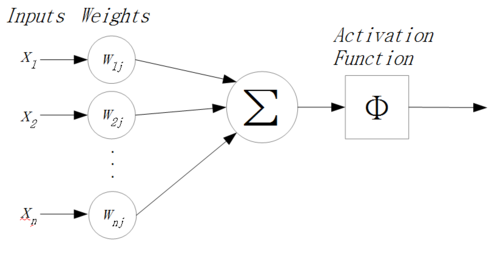
\includegraphics[width=0.7\linewidth]{./images/mcculloch-pitts.png}
		\caption{The McCulloch-Pitts neuron}
		\label{fig:m-p-neuron}
	\end{figure}\\
	The architecture of the model described in the paper was that of a multi-layer perceptron (MLP). This is a neural network made up of only dense layers\cite{intro-to-nn}. The MLP described was made up of: an input layer; a single hidden layer with $H$ neurons; and an output layer (Fig. \ref{fig:mlp-fig}). The hyper-parameter $H$ was optimized using grid search where $H \in \{0, 2, 4, 6, 8\}$. The model was trained using the BFGS\cite{bfgs} optimizer algorithm for 100 epochs, the default for the \texttt{nnet} package, the neural network package used by RMiner.
	\begin{figure}[h]
		\centering
		\includegraphics[width=0.7\linewidth]{./images/mlp-coloured.png}
		\caption{Multi-layer Perceptron architecture used in this problem}
		\label{fig:mlp-fig}
	\end{figure}
	
\subsubsection*{Code Development}
	Code for this model was initially planned to be developed using the just the Keras API with a TensorFlow backend. However Keras has no built in BFGS optimizer. For this reason TensorFlow was used, and the Keras API was accessed through it as \texttt{tf.keras}. As the paper did not specify the loss function the mean squared error (MSE) was used\footnote{Implemented using \texttt{tf.keras.losses.MeanSquaredError()}} as it is the default for RMiner. The \texttt{tfp.optimizer.bfgs_minimize} function from the TensorFlow Probability library was used to minimize the loss function of the model. This function takes two positional arguments:
	\begin{itemize}
	\item \textbf{\texttt{value_and_gradients_function}}: A Python callable which takes a single 1D tensor of variables as input and returns the value of the function to be minimised and its gradient for that input tensor.
	\item \textbf{\texttt{initial_position}}: The starting position of the variables.
	\end{itemize}
	Initially the BFGS optimizer was planned to be made by inheriting from the Keras \texttt{Optimizer} abstract\footnote{While Python does not have abstract classes this is effectively an abstract class used to define all optimizer's behaviour} class and implementing the required methods. However this design decision was changed later as \texttt{bfgs_minimize} made it difficult to implement the required functions due to it not returning intermediate values. Another problem encountered was the fact that this function uses a single 1D tensor for the variable of the function, while the model uses multiple 2D tensors for the weights of the MLP. To solve this the 4 'weight' tensors\footnote{2 weight matrices  and 2 bias vectors} were mapped to and from a 1D tensor using TensorFlows \texttt{dynamic_stitch} and \texttt{dynamic_partition}. A blog post by Py Chuang implementing a similar optimizer was used as reference\cite{pychoa-optimizer} for creating the value_and_gradient function. \par
	For my implementation I decided to extend \texttt{tf.keras.Sequential} to create a \texttt{BfgsMlp} class, which creates MLP with a single hidden layer. This overrides the \texttt{fit} method from \texttt{Sequential} to use the \texttt{bfgs_minimize} optimizer. A number of extra methods were also added to facilitate its use:
	\begin{itemize}
		\item \textbf{\texttt{_make_val_and_grad_func(self, X, y)}}: A factory function to make the value_and_gradient function , which calculates the loss and gradient of the error surface for presentations X with labels y.
		\item \textbf{\texttt{_update_weights(self, weights_1d)}}: Updates the model weights using a 1D tensor calculated by the optimizer
		\item \textbf{\texttt{_get_weights_1d(self)}}: Gets the current weights for the model mapped to a 1D tensor
		\item \textbf{\texttt{_make_1d_mapping(self)}}: Called by \texttt{__init__} to create a mapping to and from a 1D tensor for the model weights.
	\end{itemize}
	Using this model the hyper-parameter $H$ was then tuned using 10-fold cross-validation accuracy as the performance metric on which the best value of $H$ was judged (Table \ref{tab:bfgs-results}). Once the best value of $H$ was determined, it was desired to monitor the progression of the training and validation loss and accuracy over the 100 epochs, to see if over-fitting was occurring. There was a problem with this however, as the BFGS optimizer does not return intermediate values, and weights need to be updated in the \texttt{value_and_gradient} function. Therefore to monitor the intermediate loss and accuracy of the model, a new class, \texttt{BfgsTrainingMonitor}, was made. This takes the model and the datasets you want to test the model with each epoch, i.e. the training and validation datasets. This monitor can then be passed to the \texttt{BfgsMlp.fit function}, and uses a wrapper function \texttt{monitor(func)} to wrap the \texttt{value_and_gradient} function for the model. It then calls the models \texttt{evaluate(X, y)} function, and records the results for the metrics returned in a Python dictionary. This was used to create graphs to show how the accuracy and loss change by epoch, see Figure~\ref{fig:nn-loss-acc}. There was one issue with this method however, which is that the value_and_gradient function appears to be called 3 times per iteration of the bfgs algorithm. No reason could be found for this in either the TensorFlow Probability documentation for this function, or its source code. \par
	From these graphs it can be seen that after around 40 epochs the training loss continues to reduce while the validation loss begins increasing. This is a common sign that the model is overfitting and learning the noise of the training data, rather than the underlying information\cite{overfitting}. Using 40 epochs and 4 hidden neurons, 5 final models were trained on 90\% of the Portuguese data, and validation accuracy calculated using the other 10\% of the data. The best model was then tested against the Maths data.
	
	\begin{figure}[h]
		\centering
		\begin{subfigure}{0.5\textwidth}
	  		\centering
  			\includegraphics[width=\linewidth]{./images/nn-loss.png}
  			\caption{Training vs. Validation loss}
  			\label{fig:nn-loss}
		\end{subfigure}%
		\begin{subfigure}{0.5\textwidth}
  			\centering
	  		\includegraphics[width=\linewidth]{./images/nn-acc.png}
  			\caption{Training vs. Validation accuracy}
 			\label{fig:nn-acc}
		\end{subfigure}
		\caption[LLL]%
		{Training history for BfgsMlp with $H = 4$\footnotemark}
		\label{fig:nn-loss-acc}
	\end{figure}
	\footnotetext{Note No. calls to \texttt{val_and_grad_func} is $3\times$ the number of epochs}

\subsubsection*{Results}
	Table \ref{tab:bfgs-results} shows the mean validation accuracy with 10-fold cross-validation for the MLP using BFGS optimization for 100 epochs with various numbers of hidden nodes, $H$. it can be seen that the validation accuracy peaks when $H = 4$, at 67.85\%. This value of $H$ was then used by 5 models trained for 40 epochs to prevent over-fitting. The best performing model achieved a validation accuracy of 75.38\%. This model was then tested against the student maths dataset, and achieved 65.32\%, showing that it was able to generalise to unseen data.
	
	\begin{table}[h]
		\centering
		\begin{tabular}{|r| c c c c c|}
			\hline
			\textbf{H}	& 0 & 2 & 4 & 6 & 8 \\ \hline
			\textbf{Accuracy} & 28.92\% & 66.15\% & 67.85\% & 62.15\% & 64.62\%  \\ \hline
		\end{tabular}
		\caption{Results of tuning H}
		\label{tab:bfgs-results}
	\end{table}
	

\subsection{Support Vector Machine}

\subsubsection*{Overview}
	Support vector machines (SVM) were first described in 1995 by Corinna Cortes and Vladimir Vapnik in their paper \textit{Support-Vector Networks}\cite{support-vector-machines}. They are a popular machine learning algorithm as they reach a global optimum by maximising the distance between data points and the decision boundary. SVM allow for binary classification, though a multi-class SVM can be made from the combination of multiple binary SVMs, or using multi-class kernel-based vector machines\cite{multiclass-svm}. An SVM can only solve linearly-separable problems, which limits their usefulness, however through the use of the \textit{'kernel trick'}\cite{ml-algorithmic-perspective}, they can solve much more complex, non-linearly solvable  problems. This is done by using a kernel function to map the features into some higher dimensional space, where they are linearly-separable. \par
	SVM offer a number of hyper-parameters, such as: \textbf{$C$} a 'slack' variable; and $\gamma$ a parameter used by the kernel functions. Only $\gamma$ was tuned in the original paper, where $\gamma \in \{2^{-9}, 2^{-7}, 2^{-5}, 2^{-3}, 2^{-1}\}$. The slack variable $C$ was left as the default value of 1, which is also the default in Scikit-Learn. No kernel was mentioned in the original paper, so several kernel functions were looked at: Radial-bias function (RBF); Sigmoid; Polynomial (degree 3); and linear, which does not map the data-points to a higher dimensionality space. No form of dimensionality reduction for the data such as principle component analysis (PCA) was looked at either, though it has been shown that removing features with little correlation to the labels can improve SVM classification performance\cite{svm-reduce-dim}. For this reason it was looked at to demonstrate Scikit-Learns various dimensionality reduction methods, and to see if it has any improvement on classification accuracy.
	
\subsubsection*{Code Development}
	Code for this model was made using Scikit-Learn's \texttt{sklearn.svm.SVC} class. To tune the $\gamma$ value, scikit-learn's \texttt{sklearn.model_selection.GridSearchCV} was used. This allows for a user to tune a models hyper-parameter using a grid-search method, i.e. checking all combinations of hyper-parameters, and using k-fold cross-validation to measure performance. Hyper-parameters are given in a Python dictionary, along with an instance of the type of model to use and some training data. Once training of the models is done, information about the results can be accessed, along with the best performing model, and other various information about the training process. For this grid-search, both the $\gamma$ value and the kernel functions were varied. The results for this can be seen in Tables \ref{tab:no-pca-tab} -- \ref{tab:scree-pca-tab} in the SVM results section. 
	Next the affect of reducing dimensionality on the accuracy of the classification was looked at. For this a number of PCA algorithms were looked at. Principle component analysis, as the name suggests, looks at the variance captured in each feature, and continues to take the feature which represents the most variance, until a certain threshold is reached\cite{pca}. The remaining features are then discarded, and the the selected features used as the new dataset. This also corresponds to taking the $q$ largest eigenvectors of the data's covariance matrix, and this the method implemented by Scikit-Learn. There are numerous ways to select how many PCs should be used, such as Kaiser's stopping rule or the scree test\cite{pca-choosing-2}. Kaiser's stopping rule states that only factors with an eigenvalue of greater than $1.00$ should be used\cite{pca-choosing}. Table~\ref{tab:kaiser-tab} shows the 11 largest eigenvalues, of which 10 would be used as they are greater than $1$. The scree test takes a more graphical approach to this, by plotting the features vs. their eigenvalues in descending order, it can be seen when the eigenvalues level out, and this is taken as the cut-off\cite{pca-choosing}, as seen in Figure~\ref{fig:scree-test}, this happens after the first 3 features. An identical approach was then used to performing hyper-parameter tuning for the models using datasets of these reduced dimensions.\\
	\begin{minipage}[h]{\textwidth}	
		\begin{minipage}{0.3\textwidth}
		\begin{table}[H]
			\centering
			\begin{tabular}{|r|r|}
				\hline
				\textbf{Factor} & \textbf{Eigenvalue} \\ \hline
				1	&	3.8335 \\
				2	&	2.5561 \\
				3	&	1.7764 \\
				4	&	1.5177 \\
				5	&	1.4267 \\
				6	&	1.3117 \\
				7	&	1.2629 \\
				8	&	1.1248 \\
				9	&	1.0694 \\
				10 	&	1.0327 \\
				11	&   0.9958 \\
				\hline
			\end{tabular}
			\caption {Factors and Eigenvalues} 
			\label{tab:kaiser-tab} 
		\end{table}
		\end{minipage}%
		\hspace{0.6cm}%
		\begin{minipage}{0.7\textwidth}
		\begin{figure}[H]
			\centering
			\vspace{0.9cm}
			\includegraphics[width=\textwidth]{./images/scree-test.png}
			\caption{Scree Test showing factor vs. eigenvalue. Notice the drop off after 3 factors}
			\label{fig:scree-test}
		\end{figure}
		\end{minipage}
	\end{minipage} \\
	
\subsubsection*{Results}
	For the first test ,not using PCA on the data, it was found that setting the kernel to 'linear', i.e. using no kernel function, got the best result and was closest to the result in the original paper, with a mean accuracy of $67.62\% \pm4.8$. This is unexpected, as the best model with a kernel function only had a mean accuracy of $51.73\% \pm4.3$, with a $\gamma$ of 0.002. It also means that $\gamma$ was unused by the best model, so tuning it was not needed. It can also be seen for all data inputs, Tables \ref{tab:no-pca-tab} -- \ref{tab:scree-pca-tab}, that for $\gamma < 2^{-5}$ no difference was seen in accuracy for any kernel. After this the best model from each grid-search\footnote{Using the full data, the kaiser selected components and the scree selected components} was tested against the maths dataset, and the following accuracies measured (Table \ref{tab:svm-maths-acc}). \\
	
	\begin{table}[h]
		\centering
		\begin{tabular}{|ll|ccccc|}
			\hline
                                      &                                      &   			& \multicolumn{3}{c}{\textbf{Gamma $\boldsymbol{\gamma}$}} &   \\ \hline
                                      &                                      				& $2^{-9}$  		& $2^{-7}$       	& $2^{-5}$      	& $2^{-3}$			& $2^{-1}$ \\ \hline
			\multicolumn{1}{|l|}{\textbf{Kernel}} & \multicolumn{1}{r|}{\textbf{Linear}} 	& \boldmath$67.62\%$ 	& --  	& --				& --	  			& --			   \\
			\multicolumn{1}{|l|}{\textbf{}}       & \multicolumn{1}{r|}{\textbf{RBF}}    	& $31.84\%$ 	& $31.84\%$  & $31.84\%$  & $45.23\%$  & $32.37\%$ \\
			\multicolumn{1}{|l|}{\textbf{}}       & \multicolumn{1}{r|}{\textbf{Poly}}   	& $31.84\%$ 	& $31.84\%$  & $31.84\%$  & $31.84\%$  & $50.02\%$ \\
			\multicolumn{1}{|l|}{\textbf{}}       & \textbf{Sigmoid}                     	& $31.84\%$ 	& $31.84\%$  & $31.84\%$  & $38.00\%$  & $51.73\%$ \\ \hline
		\end{tabular}%
		\caption {Results using no PCA (Best accuracy in bold)} 
		\label{tab:no-pca-tab} 
	\end{table}
	
	\begin{table}[h]
		\centering
		\begin{tabular}{|ll|ccccc|}
			\hline
                                      &                                      &   			& \multicolumn{3}{c}{\textbf{Gamma $\boldsymbol{\gamma}$}} &   \\ \hline
                                      &                                      				& $2^{-9}$  		& $2^{-7}$       	& $2^{-5}$      	& $2^{-3}$			& $2^{-1}$ \\ \hline
			\multicolumn{1}{|l|}{\textbf{Kernel}} & \multicolumn{1}{r|}{\textbf{Linear}} 	& \boldmath$56.51\%$ 	& --  	& --				& --	  			& --			   \\
			\multicolumn{1}{|l|}{\textbf{}}       & \multicolumn{1}{r|}{\textbf{RBF}}    	& $31.84\%$ 	& $31.84\%$  & $31.84\%$  & $41.81\%$  & $47.93\%$ \\
			\multicolumn{1}{|l|}{\textbf{}}       & \multicolumn{1}{r|}{\textbf{Poly}}   	& $31.84\%$ 	& $31.84\%$  & $31.84\%$  & $31.84\%$  & $46.75\%$ \\
			\multicolumn{1}{|l|}{\textbf{}}       & \textbf{Sigmoid}                     	& $31.84\%$ 	& $31.84\%$  & $31.84\%$  & $37.66\%$  & $48.29\%$ \\ \hline
		\end{tabular}%
		\caption {Results using Kaiser PC selection (Best accuracy in bold)} 
		\label{tab:kasier-pca-tab}
	\end{table}
	
	\begin{table}[h]
		\centering
		\begin{tabular}{|ll|ccccc|}
			\hline
                                      &                                      &   			& \multicolumn{3}{c}{\textbf{Gamma $\boldsymbol{\gamma}$}} &   \\ \hline
                                      &                                      				& $2^{-9}$  		& $2^{-7}$       	& $2^{-5}$      	& $2^{-3}$			& $2^{-1}$ \\ \hline
			\multicolumn{1}{|l|}{\textbf{Kernel}} & \multicolumn{1}{r|}{\textbf{Linear}} 	& $45.54\%$ 	& --  				& --				& --	  			& --			   \\
			\multicolumn{1}{|l|}{\textbf{}}       & \multicolumn{1}{r|}{\textbf{RBF}}    	& $31.84\%$ 	& $31.84\%$  & $31.84\%$  & $40.77\%$  & \boldmath$46.39\%$ \\
			\multicolumn{1}{|l|}{\textbf{}}       & \multicolumn{1}{r|}{\textbf{Poly}}   	& $31.84\%$ 	& $31.84\%$  & $31.84\%$  & $31.84\%$  & $42.47\%$ \\
			\multicolumn{1}{|l|}{\textbf{}}       & \textbf{Sigmoid}                     	& $31.84\%$ 	& $31.84\%$  & $31.84\%$  & $37.14\%$  & $33.08\%$ \\ \hline
		\end{tabular}%
		\caption {Results using Scree PC selection (Best accuracy in bold)} 
		\label{tab:scree-pca-tab}
	\end{table}
	
	\begin{table}[h]
		\centering
		\begin{tabular}{|r| c c c|}
			\hline
			\textbf{Component selection}	& All		& Kaiser	& Scree \\ \hline
			\textbf{Accuracy}				& 10.13\%	& 10.13\%	& 26.03\% \\ 
			\hline
		\end{tabular}
		\caption{Accuracies of best models on maths data using different component selections}
		\label{tab:svm-maths-acc}
	\end{table}		
	
	As mentioned, removing features from the data with little correlation can improve the accuracy of SVMs. For this data however this was not the case, both Kaiser and Scree principle component selections achieved worse accuracy on the Portuguese data. On the maths data none of the models performed well, with only the model using the 3 scree selected components performing better than random guessing with an accuracy of 26\%. This most likely means that the SVMs were learning some underlying data that did not correlate well between maths and Portuguese. 
	However there is another benefit of reducing dimensionality, which is the reduction to training times. Using the full 32 features of the training set, it took 0.04 seconds to train and model using a linear kernel on average, compared to 0.014 seconds when using 10 features and 0.009 seconds when using 3 features. While for a dataset of this size training time is not an issue, for datasets that could have over a 100,000 presentations this could represent reasonable trade-off in accuracy for training time, especially if features with low variance exist in the dataset.
	
\subsection{Decision Tree}
	
\subsubsection*{Overview}
	Binary trees are a very common and well studied data-structure in computer science. Searching through a balanced binary tree is very efficient, $O(\log N)$, where $N$ is the number of nodes. Decision trees are binary trees constructed to classify data based on features\cite{ml-algorithmic-perspective}. This makes them very fast for querying once they have been constructed. There are a number of algorithms for constructing decision trees, such as ID3\cite{ID3} or CART\cite{CART}. These are usually greedy algorithms that focus on trying to separate the features to split the classes the most evenly. To do this they use some measure of informational entropy, which measures how much the data can be split by a single feature, which is a maximum when it splits the data is split in half\cite{info-entropy}. \par
	The default entropy function used by the \texttt{rpart} models, the decision tree package used by \texttt{rminer} is Gini impurity, Eqn.~\ref{eqn:gini}, which is the entropy measurement used by CART. This function computes the \textit{'purity'} of a node, where a pure node is one that corresponds to a single class $i$ in the dataset, if that node where to split the data based on some feature $k$. If we count the number of data points $N(i)$ then we can calculate the Gini impurity as:
	\begin{equation}
	G_k = 1 - \sum_{i=1}^c N(i)^2
	\label{eqn:gini}
	\end{equation}
	Along with the criterion function on which nodes are split, there are a number of other hyper-parameters that can be used to improve decision tree performance. Of particular importance to preventing over-fitting are the maximum depth of the decision tree, and the \textit{complexity parameter} used in minimal cost-complexity pruning. The maximum depth, as the name suggests, simply limits the maximum number of layers a decision tree can have. This stops the tree from splitting features too many times to try and correctly classify every point. Minimal cost-complexity pruning is an algorithm for pruning nodes from trees to minimise $R_\alpha(T)$, where $\alpha \geq 0$ is the complexity parameter (Eqn.~\ref{eqn:ccp}). Here $R(T)$ is the is the total misclassification rate of tree $T$, and $|T|$ is the number of terminal nodes in $T$.
	\begin{equation}
		R_\alpha(T) = R(T) + \alpha|T|
	\label{eqn:ccp}
	\end{equation}
	
\subsubsection*{Code Development}
	For tuning the max depth and the complexity parameter of the decision tree \texttt{GridSearchCV} was again used. While \texttt{rpart} supports both of these hyper-parameters, it does not have default values for them, and none was mentioned in the paper. For this reason the grid-search was set to tune the \texttt{max_depth} and the \texttt{ccp_alpha} hyper-parameters of the \texttt{DecisionTreeClassifier} from Scikit-learn. The max depth was tried with 3 different values, 3, 5, and None. For the complexity parameter two values were tested, 0, and the optimal $\alpha$ value. The optimal $\alpha$ value was calculated as follows:
	
	\begin{enumerate}
	\item Using \texttt{DecisionTreeClassifier.cost_complexity_pruning_path(X, y)} the effective $\alpha$ of each node in a tree can be calculated. This is the $\alpha$ at which the node would be pruned from the tree. 
	\item From these effective alphas we can create DTs using these values and plot the number of nodes and depth of the tree's against $\alpha$, as seen in Figure~\ref{fig:alpha-nodes-depth}, the depth and number of nodes quickly drop off as $\alpha$ increases.
	\item Using these models we can also plot the training and validation accuracy against $\alpha$, as seen in Figure \ref{fig:alpha-accuracy}. From this the best $\alpha$ to prevent over-fitting can be seen to be around 0.005. This value maximises validation accuracy, and as seen in Figure~\ref{fig:alpha-nodes-depth} also reduces the number of nodes and the depth drastically, improving generalisation of the trees.
	\end{enumerate}
	
	The two best trees were then graphed using \texttt{sklearn.tree.export_graphviz} and \texttt{graphviz}. These can be seen in Figures \ref{fig:dt-no-ccp} and \ref{fig:dt-ccp}. These offer an easy way to see how the data is being split at each node, and the effect of cost-complexity pruning on a decision tree\footnote{A full page version of these trees can be seen in the appendix, as they are quite large}. The colour each node corresponds to the dominant class at that node, with shade corresponding to the proportion of data points of that class at that node. From these it can be seen how cost-complexity pruning reduces the number of terminal nodes.
	
	\begin{minipage}[t]{\textwidth}
	\begin{minipage}{0.5\textwidth}
		\centering
		\begin{figure}[H]
	  		\centering
  			\includegraphics[width=\linewidth]{./images/node-alpha.png}
  			\caption{$\alpha$ vs. Size of tree}
  			\label{fig:alpha-nodes-depth}
		\end{figure}
	\end{minipage}%
	\hspace{0.5cm}%
	\begin{minipage}{0.5\textwidth}
		\begin{figure}[H]
  			\centering
	  		\includegraphics[width=\linewidth]{./images/alpha-acc.png}
  			\caption{$\alpha$ vs. Training and Validation accuracy}
 			\label{fig:alpha-accuracy}
		\end{figure}
	\end{minipage}%
	\hspace{0.5cm}
	\end{minipage}
	
	\begin{figure}[h]
		\centering
  		\includegraphics[width=\linewidth]{./images/dt-no-ccp.png}
  		\caption{Best decision tree without pruning}
  		\label{fig:dt-no-ccp}
	\end{figure}
	
	\begin{figure}[h]
		\centering
  		\includegraphics[width=\linewidth]{./images/dt-ccp.png}
  		\caption{Best decision tree with pruning}
  		\label{fig:dt-ccp}
	\end{figure}
	
\subsubsection*{Results}
	The results from the hyper-parameter grid-search using 10-fold cross-validation can be seen below, Table \ref{tab:dt-results}. From this a number of observations can be made about the effect of both the max depth and $\alpha$ value have on a decision tree's accuracy and training time. The first observation is that both limiting the max depth and using cost-complexity pruning improve validation results greatly. Without pruning limiting the max depth improves validation accuracy by around 14\%, and without limiting the depth pruning improves the validation accuracy by around 11\%. However it is also seen that the combination of limiting depth and pruning does not improve the validation much compared to the use of just on of these techniques, only around 0.5\%. 
	
	\begin{table}[h]
		\centering
		\begin{tabular}{|c|c|c|c|c|}
			\hline
			\textbf{Max Depth} 	& $\boldsymbol{\alpha}$ & \textbf{Mean fit time} (s) 	& \textbf{Mean accuracy} 	& \textbf{Standard deviation}	\\ 
			\hline
			3					& 0			& 0.0000						& 75.83\%					& 5.6\%	\\
			5					& 0			& 0.0020						& 68.28\%					& 6.5\%	\\
			--					& 0			& 0.0038						& 61.25\%					& 9.2\% \\
			\textbf{3}			& \textbf{0.005}& \textbf{0.0025}			& \textbf{76.34\%}			& \textbf{5.8\%} \\
			5					& 0.005		& 0.0032						& 73.93\%					& 7.2\% \\
			--					& 0.005		& 0.0050						& 72.38\%					& 9.1\% \\
			\hline
		\end{tabular}
		\caption{GridSearchCV results}
		\label{tab:dt-results}
	\end{table}
	
	The best model with and without pruning were then evaluated using the unseen maths dataset. With pruning an accuracy of 74.94\% was measured on the unseen data, compared to 71.39\% with pruning.
	
\subsection{Random Forest}

\subsubsection*{Overview}
	Random forests are a type of ensemble learner made up of decision trees. Ensemble learners work by taking a large number, of weak learners\footnote{A weak learner is a model whose accuracy is slightly better than chance}, each classifying the data in a different way, and combining there predictions using some algorithm\cite{ml-algorithmic-perspective}. To create a random forest the method of training the decision trees is modified slightly. Now when a node is expanded only some subset of features $m$ is considered to split the data on. The trees are then trained and combined using bootstrap-aggregation, also known as bagging. Bootstrapping involves taking some random subset of the dataset with replacement. A number of these bootstrap samples are combined to produce a new dataset of the same size as the original dataset, but that may now contain duplicates. \par
	Again the original paper used the defaults for training the RF. The RF used by \texttt{rminer} comes from the \texttt{randomForest} package in R. This defaults to 500 trees, and a minimum node size of 1 for classification. Node size refers to the number of data points associated with a node. This parameter is equivalent to the \texttt{min_samples_leaf} in Scikit-learn's \texttt{RandomForestClassifier}. However the size of the trees can also be limited by the \texttt{max_depth} parameter. Scikit-learn uses 100 trees with no max depth if the default options are used. It was decided to see how 100 trees perform in this task compared to 500. As neither library limits the size of the trees by default, and producing 100's of large trees can take significant time, it was decided to also seem how limiting the size of the trees using both \texttt{max_depth} affected the accuracy. This was checked using a grid-search method, as with the previous models.
	
\subsubsection*{Code Development}
	As hyper-parameters were to be tuned using a grid-search method, \texttt{GridSearchCV} was again used. The \texttt{min_samples_leaf} argument can take either an integer value, or a float, depending on if it should be interpreted as the absolute number or a proportion of the total dataset. Here the hyper-parameters to be tuned were $\texttt{n_estimators} \in \{100, 500\}$, and $\texttt{max_depth} \in \{3, \texttt{None}\}$.
	Graphing some of the trees produced, Figure \ref{fig:rf-dts}, it can be seen that now many more features are considered for splitting compared to when just using a single decision tree, which mainly used just $G1$ and $G2$.
	
	\begin{figure}[h]
		\centering
		\includegraphics[width=\textwidth]{./images/rf-dt-2.png}
		\caption{Two of the decision trees making up a random forest}
		\label{rf-dts}
	\end{figure}
	
	
\subsubsection*{Results}
	The results from the grid-search cross-validation can be seen below. Of note is the fact that while limiting limiting the size of the trees generated reduced the fitting time by around 20\%, not limiting the size, and reducing the number of tress not only reduced the training time by around 75\%, but also achieved a slightly better validation accuracy. The best tree was then tested on the unseen maths data and an accuracy of 64.81\%.

	\begin{table}
		\centering
		\begin{tabular}{|c|c|c|c|c|}
			\hline
			\textbf{Max Depth} 	& \textbf{No. Estimators} & \textbf{Mean fit time} (s) 	& \textbf{Mean accuracy} 	& \textbf{Standard deviation}	\\ 
			\hline
			3 		& 100 	& 0.165 	& 67.03\%  & 5.4\% \\
			3 		& 500 	& 0.845 	& 68.42\%  & 5.5\% \\
			None 	& 100 	& 0.214 	& 69.48\%  & 5.3\% \\
			None 	& 500 	& 1.076 	& \textbf{71.32\%}  & 6.6\% \\
			\hline
		\end{tabular}
		\caption{GridSearchCV results}
		\label{tab:rf-results}
	\end{table}
	
\subsection{Comparison of Results}
	Comparing the results from the NN, SVM, DT, and RF implementations, using Python frameworks Scikit-learn and Tensorflow following the original paper using R, and implementing extra techniques (Table \ref{tab:student-results-compare}) it can see that both using R frameworks and Python frameworks achieves comparable results. Table \ref{tab:student-results-compare} also shows that of the three models in which extra techniques were explored, only the limiting of the Decision tree's size had a positive impact on accuracy.
	
	\begin{table}[h]
		\centering
		\begin{tabular}{|r| c c c c|}
			\hline
			\textbf{Model}  					& NN				& SVM				& DT						 & RF		\\ \hline
			\textbf{R}	    					& 65.1\%			& 64.5\%			& 76.1\%					 & \textbf{73.5\%}	\\
			\textbf{Python}						& 67.9\%			& \textbf{67.6\%}	& 75.8\%					 & 71.4\%	\\
			\textbf{Python + modifications}		& \textbf{75.38\%}	& 51.7\%			& \textbf{\underline{76.3\%}}& 68.4\%	\\
			\hline
		\end{tabular}
		\caption{Overall results for all implementations, best per model type in \textbf{bold}, best overall \underline{underlined}}
		\label{tab:student-results-compare}
	\end{table}
	
	All these models, trained on the Portuguese dataset, were then tested using the maths dataset. This was not done by the original paper, in which each dataset was used to train its own models. A comparison of the models trained on the Portuguese data and ones trained on the maths data can be seen below in Table \ref{tab:student-maths}. From this it can be seen that having more data from a different school subject did not help to improve performance at predicting maths results for SVM, DT, or RF models. It did however improve the accuracy for the NN. The SVM did not generalise well between the two subjects, which may indicate it was over-fitted to the Portuguese data.
	
	\begin{table}
		\centering
		\begin{tabular}{|r| c c c c|}
			\hline
			\textbf{Model} 					& NN				& SVM				& DT				& RF				\\ \hline
			\textbf{Trained on Maths}		& 60.3\%			& \textbf{59.6\%}	& \textbf{76.7\%}	& \textbf{72.4\%}	\\
			\textbf{Trained on Portuguese}	& \textbf{65.3\%}	& 26\%				& 74.9\%			& 64.81\%			\\
			\hline
		\end{tabular}
		\caption{Comparison of model accuracy with maths dataset when trained on maths vs. Portuguese}
		\label{tab:student-maths}
	\end{table}

	Overall this example problem shows that the Python frameworks Scikit-learn and TensorFlow have comparable performance to the R RMiner framework. It also shows that a number of machine learning techniques, such as dimensionality reduction, cross-validation, grid-search parameter tuning, and decision tree pruning are easily performed using Scikit-learn. It was also seen that while TensorFlow already has many standard optimizers implemented already, it is also possible use custom optimizers from different Python libraries. 


\chapter{Problem 2: Detecting Pneumonia}
\section{Problem Overview}
	% Explanation of pneumonia
	Pneumonia is an inflammation of the lungs which can be caused by either a fungal, bacterial or viral infection. Of these bacterial or viral infection are the more common cause\todo{source}. According to the \textit{The European Lung white book; Respiratory Health and Disease in Europe} it had a mortality rate in Ireland of 32.96 per 100,000 in 2011\cite{pne-death-rate}, which, when compared to the total death rate in Ireland for 2011 of 6.2 per 1,000, means that pneumonia was responsible for 5.3\% of deaths in Ireland in 2011. \par
	% Diagnosis mehtods and use of deep learning in medicine
	There are a number of methods to reliably rule in or out pneumonia when diagnosing a patient, such as the lack of certain symptoms or the presence of rates and bronchial breathing sounds, but chest radiography is generally considered the best method of confirming a pneumonia diagnosis\cite{pne-diagnosis}. Computer aided diagnosis (CAD) is already used for a number of diseases, including pneumonia\cite{cad-wavelet}. Most of these CAD models focus on the use of machine vision techniques rather than machine learning approaches. However, in recent years there has been a great amount of research into the use of deep learning in medical diagnosis, in particular for use image-based diagnosis, such as MRI, CAT or X-Rays\cite{pne-ml-in-medicine}. These models are often able to achieve comparable, or sometimes higher, detection rates of these diseases compared to doctors, making them very useful tools. \par
	% Details on dataset
	This example problem aims to demonstrate how a machine learning model could be developed for detecting pneumonia from chest x-rays. A number of deep learning methods will be explored, but only convolutional neural network (CNNs) models will be used, as almost all real world models for image-based medical diagnosis use CNNs\cite{pne-ml-in-medicine}. \par

\section{Convolutional Neural Networks}
	% Explanation of CNNs
	Convolutional neural networks (CNNs) are a class of neural networks which use convolutional layers to extract translation invariant \textit{features} from an \textit{feature map}, which can be any matrix $m \in \mathbb{R}^{w \times h \times d}$\cite{cnn-analysis}, such as an image. These features can then be passed as a vector to a neural network and the neural network can then be trained as usual. CNN classification models can generally be broken up into two distinct blocks of layers; a set of layers for feature extraction, and a set of layers for classification. \par
	\begin{figure}[h!]
  		\centering
  		\includegraphics[width=0.7\linewidth]{./images/cnn-block-diagram.png}
  		\caption{Block diagram of typical CNN}
  		\label{fig:cnn-block}
	\end{figure}
	Despite being shown to be effective at solving machine vision tasks and fully trainable by back-propagation since 1989\cite{cnn-backprop}, it was not until as recently as 2012, when a CNN achieved a top-5 test error rate of 15.3\%, compared to next highest of 26.3\% in the ImageNet challenge\cite{cnn-image-net} that they were considered state-of-the-art. \par
	
	% Explanation of layers and keras implementations
	There are three types of layer typically found in the feature extraction block of a CNN model; Convolutional layers, pooling layers, and normalization layers\cite{cnn-analysis}. Keras\cite{keras} has a number of built in  implementations of these layers to allow their use in models.
	\subsection{Convolutional Layers}
	Similar to how perceptrons were designed to approximate the neurons in the brain, units in convolutional layers were designed to replicate the cells found in the visual cortex, which have a receptive field, and respond regions of the visual field\cite{cnn-biology}. To do this, convolutional layers use a number, $n$, of filters as their base units, which when convolved with an input feature map produce $n$ output feature maps. The filters, commonly called kernels, are matrices of weights $w \in \mathbb{R}$ of size $k_w \times k_h$ where $k_w, k_h \in \mathbb{N}_{\geq1}$\cite{cnn-analysis}.
	
%	\begin{figure}[h!]
%  		\centering
%  		\includegraphics[width=0.7\linewidth]{../final-report/images/conv-explain.png}
%  		\caption{Diagram showing convolution of kernel with feature map}
%  		\label{fig:cnn-explain}
%	\end{figure}

	This creates a number of hyperparameters needed to define a convolutional layer;
	\begin{itemize}
	\item $n$, the number of filters,
	\item $(k_w, k_h)$ the shape of the filters, typically square,
	\item the activation function for the layer, which should be non-linear (similar to a normal perceptron layer),
	\item the stride $s \in \mathbb{N}_{\geq1}$, which defines how much to move the kernel by when doing the convolutional,
	\item and the padding, which is used to determine the values convolved with the filter when it overlaps the edges of the image.
	\end{itemize}
	Keras offers a number of implementations of convolutional layers in the \texttt{keras.layers} module, covering several subtypes of convolutional layer, and with a number of arguments to set the hyperparmeters mentioned above;
	\begin{itemize}
	\item Basic convolution; basic convolutional layers with various shapes of filter, such as 1D, 2D and 3D are offered by \texttt{Conv1D}, \texttt{Conv2D} and \texttt{Conv3D} respectively.
	\item Depthwise separable convolution; when dealing with images with multiple channels, such as an RGB image, the number of multiplications done during convolution can get very large. To reduce the number of multiplications done, depthwise convolution can be done instead, convolving each channel of the image separably, and then the channels can be combined using a $1 \times 1 \times d$ kernel. This produces the same result as a regular convolution, but requires far fewer multiplications, and also fewer parameters\cite{cnn-depth-conv}. This is implemented in the keras layers \texttt{SeparableConv1D} and \texttt{SeparableConv2D}.
	\item Depthwise convolution; if only a depthwise convolution is desired, i.e. a convolution on each input channel individually without combining afterwards, then a \texttt{DepthwiseConv2D} layer can be used.
	\end{itemize}
	
	\subsection{Pooling Layers}
	Pooling is used to reduce the size of a feature map, while trying to retain the features. This is done by creating a summary of $p \times p$ areas of the image. The summary is created by applying a function to the pooled area, commonly used functions being; max pooling, taking the maximum value in the area; average pooling, taking the mean of an area; $l_2$ pooling, which takes the $l_2$ norm of the pooled area; and stochastic pooling, which selects a value for each area using its activation value to compute a probability.\cite{cnn-analysis}.
	
	\subsection{Normalization Layers}
	\todo{Not sure if worth talking about}

\section{Dataset}
	The chest x-rays used in this problem come from the \textit{Labeled Optical Coherence Tomography (OCT) and Chest X-Ray Images for Classification} dataset\cite{pne-dataset}\footnote{Version 2} produced by Daniel Kermany, Kang Zhang and Michael Goldbaumusing and is used under the Creative Commons \textit{CC BY 4.0} license. This dataset contains 5856 images split into 3 directories; a training directory of 5216 images; a testing directory containing 624 images; and a validation directory containing 16 images. Pneumonia is prevalent in around 75\% of the training presentations, and 60\% of the test presentations. \par
	The images were loaded using Keras's \texttt{ImageDataGenerator}. This acts as a Python generator, loading in images in batches as they are needed, rather than all at once. The advantage of this is that only the images in the current batch are loaded into memory, meaning large datasets don't fill up memory unnecessarily. Using an \texttt{ImageDataGenerator} also allows for various preprocessing tasks to be carried out on the images as they are loaded. \par 
	To create a dataset usable by Keras, three \texttt{ImageDataGenerator} were made, one for training data, one for validation data, and one for test data. Due to the small number of images in the validation folder, both the training and validation presentations were drawn from the training folder. The proportion of the size of the training dataset to validation dataset was controlled using the \texttt{validation_split} argument of the \texttt{ImageDataGenerator}. The training/validation generator also used shuffling to randomise the images presented in each batch. Both generators rescaled the pixel values of the images to between 0 and 1, and resized the images to $256\times256$.
	
	\begin{figure}[h]
		\centering
		\includegraphics[width=0.9\textwidth]{./images/pne-example-images.png}
		\caption{Example of x-ray with and without pneumonia}
		\label{fig:pne-example-x-rays}
	\end{figure}


\section{Explored Solutions}
	An iterative design approach was used to tackle this problem, with each iteration of the design using more advanced models and techniques.
	\subsection{Simple CNN}
	The first solution looked at was a simple convolutional neural network, based on a similar model on Kaggle\cite{cnn-simple-kaggle}. This was composed of 3 convolutional layers, with a $3\times3$ kernel size, and rectified linear activation function, each followed by a max-pooling layer, with a $2\times2$ pool size. After these convolutional layers a dense layer of 64 neurons, again using the rectified linear activation function, before a single neuron output layer, using a sigmoid activation function to create a binary classifier. A dropout layer was use to remove the effect of 50\% of neurons in the hidden layer impacting the output during training. This is done to help prevent over-fitting\cite{dropout}. \par
	Due to the unbalance nature of the classes, a dictionary of class weights was passed to the \texttt{fit} function of the model. This is used to weigh the updates to the models weights more heavily towards presentations of class 0, i.e. x-rays without pneumonia. This has the effect of effectively balancing the data. Without doing this the model simply guesses class 1 for any presentation as it has a 75\% chance of being correct. Instead of looking at accuracy during training, specificity and sensitivity were instead used as metrics. Sensitivity is the measure of the proportion of true positives identified as positives, while specificity is the measure of the proportion of true negatives identified as such. These metrics are often looked at when dealing with problems that require a low false positive or false negative rate, such as in medical diagnosis. \par
	Keras allows for callback functions to be passed to the model to allow interaction with the model during fitting. There are several built-in callbacks offering functionality such as early-stopping, check-pointing, and logging. This model was trained for 24 epochs with a batch size of 16 images. The \texttt{TensorBoard} callback was used to monitor and record the training cycle. This callback allows for the training metrics to be monitored and re-opened in an interactive locally hosted web-page, as well as a number of other visualisations of the model and its training performance. Figures \ref{fig:cnn-basic-loss} -- \ref{fig:cnn-basic-spec} show the training and validation loss, sensitivity, and specificity during training. 
	
	\begin{figure}[t]
		\centering
		\includegraphics[width=0.5\textwidth]{./images/cnn-basic-loss.png}
		\caption{Training and validation loss}
		\label{fig:cnn-basic-loss}
	\end{figure}
	
	These graphs provide some insight into the model performance. From the loss (Fig. \ref{fig:cnn-basic-loss}) it can be seen that the training loss continues to drop, while the validation loss increases, this is a common sign of the model over-fitting to the noise of the training data, rather than learning the underlying data. Comparing the sensitivity and specificity plots (Figs. \ref{fig:cnn-basic-spec} \& \ref{fig:cnn-basic-sense}), they both perform well, however the validation specificity remains much closer to the training value and is more stable than the sensitivity. This is an issue, as it implies that it has a high rate of false negatives, compared to false positives, which are relatively low on unseen data.
	
	\begin{minipage}[b]{\linewidth}
	\begin{minipage}{0.45\textwidth}
		\begin{figure}[H]
			\centering
			\includegraphics[width=\textwidth]{./images/cnn-basic-spec.png}
			\caption{Training and validation specificity}
			\label{fig:cnn-basic-spec}
		\end{figure}
	\end{minipage}%
	\hspace{1cm}%
	\begin{minipage}{0.45\textwidth}
		\centering
		\begin{figure}[H]
			\centering
			\includegraphics[width=\textwidth]{./images/cnn-basic-sense.png}
			\caption{Training and validation sensitivity}
			\label{fig:cnn-basic-sense}
		\end{figure}
	\end{minipage}%
	\end{minipage}
	
	
	\subsection{Image Augmentation}
	The issue of over-training  is a common problem for machine and deep-learning models, and often results in poor performance from the models when exposed to real-world, unseen data. A common reason for over-fitting is a lack of training data, making it easier for the model to learn the intricacies of each data-point, rather than having to learn the underlying information. Increasing the size of a dataset can often be difficult, as data, especially medical data, can be uncommon, as in the case of rare diseases, or hard to access. Instead data augmentation or warping is used to effectively create new data-points from the existing dataset\cite{image-aug-over-fitting}. This involves transforming presentations in such a way as to make a new, but still realistic presentation. \par
	Image augmentation is a type of data augmentation that involves performing transformations on the training images, to try stop the model from learning the noise in the dataset, and instead learn the desired features\cite{image-augmentation}. The hope being that by applying semi-random augmentations to the images before they are shown to the system, undesired information will become more random and the system will learn less about it. There are a number of transformations, both elastic and rigid, that may be applied to an image. The transformations that are suitable depend largely on the subject of the image. While elastic transformations have been shown to be effective for certain medical imaging tasks, such as detecting breast cancer\cite{breast-cancer-detection}, they are not suitable for images involving rigid objects, such as chest x-rays\cite{chest-xray-augmentation}. \par
	The Keras \textit{ImageDataGenerator} has a number of arguments that can be used to apply these transformations to images as they are presented. Of relevance are:
	\begin{itemize}
		\item Rotations; An integer can be passed to set the limit in degrees for random rotations to apply to the image using the \verb!rotation_range! keyword argument. As not all the x-rays are perfectly vertical, a small rotation is allowable without making an unrealistic presentation.
		\item Shifts; The image can be shifted vertically or horizontally by a random number of pixels using the \verb!width_shift_range! and \verb!height_shift_range! keyword arguments. Similar to rotations small shifts in both horizontally and vertically are acceptable.
		\item Mirroring; The image may 50\% of the time be mirrored around either the vertical or horizontal axis using the \verb!horizontal_flip! and \verb!vertical_flip! keyword arguments. As pneumonia is possible in both the right and left lung, flipping the image along the vertical axis is reasonable.
	\end{itemize}
	By using these transformations, the over-fitting issue of the simple CNN described previously can be improved, a seen in Figure \ref{fig:cnn-aug-loss}. However while the validation specificity has remained close to the training specificity (Fig. \ref{fig:cnn-aug-spec}), the validation sensitivity has become a lot more inconsistent (Fig. \ref{fig:cnn-aug-sense}), and on average dropped compared to when no image augmentation was done. This means the model is now predicting false negatives more often before, which is undesirable.
	
	\begin{figure}[t]
		\centering
		\includegraphics[width=0.5\textwidth]{./images/cnn-aug-loss.png}
		\caption{Training and validation loss}
		\label{fig:cnn-aug-loss}
	\end{figure}


	\begin{minipage}[b]{\linewidth}
	\begin{minipage}{0.45\textwidth}
		\begin{figure}[H]
			\centering
			\includegraphics[width=\textwidth]{./images/cnn-aug-spec.png}
			\caption{Training and validation specificity}
			\label{fig:cnn-aug-spec}
		\end{figure}
	\end{minipage}%
	\hspace{1cm}%
	\begin{minipage}{0.45\textwidth}
		\centering
		\begin{figure}[H]
			\centering
			\includegraphics[width=\textwidth]{./images/cnn-aug-sense.png}
			\caption{Training and validation sensitivity}
			\label{fig:cnn-aug-sense}
		\end{figure}
	\end{minipage}%
	\end{minipage}
	
	\subsection{Transfer learning}
	Now that the over-fitting issue was resolved, the erratic sensitivity and specificity issue could be looked at. The most probable reason for the inconsistent sensitivity and specificity is that there are some presentations in the validation that it doesn't classify well, so ends up guessing. This would also explain why the two metrics got worse after applying augmentation, there are now effectively more presentations it must guess on. The easiest ways to resolve this would be to allow it to train for more epochs, or to use a more powerful model, by adding more convolutional layers. \par 
	Training a more powerful model however will require more computing power, and drastically increase the time taken to train a model. Transfer learning is a common method used to bypass this problem. This is a method whereby powerful models already trained at some task are re-purposed to solve some other task. This method is common in image recognition problems and has been used for a variety of medical diagnosis models. The idea is that by taking the convolutional layers used to extract features by some powerful model trained on a vary large, highly varied dataset, such as CIFAR-100, which is a dataset with 60,000 images spread over 100 classes. A model trained on such a dataset should therefore be good at extracting a wide variety of features from images, and then feeding these features into a neural network it will be able to solve some new problem. \par 
	For this problem the VGG-16 model\cite{vgg16} was used as the basis for the model. The VGG-16 model was trained by Oxford's \textit{Visual Geometry Group} and submitted into the 2014 ImageNet challenge where it won first place in localisation and second place in classification. This is one of the reasons it was chosen as a basis for transfer learning, the other two being: it has been shown to work for detecting pneumonia before\cite{cnn-vgg16-for-pne}; and it is available through Keras. The VGG-16 model uses 18 layers for feature extraction, 13 convolutional layers and 5 max-pooling layers, as seen in Figure \ref{fig:vgg16}. \par
	
	\begin{figure}[h]
		\centering
		\includegraphics[width=\textwidth]{./images/vgg-16-summary.png}
		\caption{Feature extraction section of VGG-16}
		\label{fig:vgg16}
	\end{figure}
	
	Using Keras these layers can be loaded in with a number of options, such as the input shape, and whether to initialise the weights randomly or to the weights when the model was trained on ImageNet. For this model the ImageNet weights were used and the input shape was set to $256 \times 256 \times 3$. This resulted in 14.7 million parameters. These weights were then fixed to speed up training by looping over the layers and setting \texttt{layer.trainable = False}. To then classify the extracted features a dense layer with 256 neurons using \texttt{relu} activation were used. A \texttt{dropout} layer was then used to apply a dropout of 0.5 before a single neuron using a sigmoid activation function was used for binary classification (Fig. \ref{fig:transfer-summary}.
	
	\begin{figure}[h]
		\centering
		\includegraphics[]{./images/transfer-summary.png}
		\caption{Transfer learning model architecture}
		\label{fig:transfer-summary}
	\end{figure}
	
	When fitting this time two new callbacks were also passed to the model, \texttt{ReduceLROnPlateau} and \texttt{EarlyStopping}. \texttt{ReduceLROnPlateau} is used to monitor some metric of the model, in this case validation loss, and if no improvement is seen in a certain number of epochs to reduce the learning rate. This is done as models often benefit from a reduction in learning rate once training stagnates, which is likely to happen sooner with a more powerful model. \texttt{EarlyStopping} is used to stop the model training if no improvement to validation loss is seen in a certain number of epochs, in this case 5 epochs. This helps to prevent over-fitting, which can happen quickly with very deep models. The model was then trained using the Adam optimizer for 32 epochs, but training was stopped by \texttt{EarlyStopping} after 10. Figures \ref{fig:cnn-trans-loss} -- \ref{fig:cnn-trans-lr} show how the loss, sensitivity, specificity, and learning rate change during training. \par
	
	\noindent\makebox[\textwidth]{
	\begin{minipage}[b]{\linewidth}
	\begin{minipage}{0.5\textwidth}
		\begin{figure}[H]
			\centering
			\includegraphics[width=\textwidth]{./images/cnn-trans-loss.png}
			\caption{Training and validation loss}
			\label{fig:cnn-trans-loss}
		\end{figure}
	\end{minipage}%
	\hspace{0.5cm}
	\begin{minipage}{0.5\textwidth}
		\begin{figure}[H]
			\centering
			\includegraphics[width=\textwidth]{./images/cnn-trans-sense.png}
			\caption{Training and validation sensitivity}
			\label{fig:cnn-trans-sense}
		\end{figure}
	\end{minipage}
	\vspace{0.5cm}
	\begin{minipage}{0.5\textwidth}
		\begin{figure}[H]
			\centering
			\includegraphics[width=\textwidth]{./images/cnn-trans-spec.png}
			\caption{Training and validation specificity}
			\label{fig:cnn-trans-spec}
		\end{figure}
	\end{minipage}%
	\hspace{0.5cm}%
	\begin{minipage}{0.5\textwidth}
		\begin{figure}[H]
			\centering
			\includegraphics[width=\textwidth]{./images/cnn-trans-lr.png}
			\caption{Learning rate during training}
			\label{fig:cnn-trans-lr}
		\end{figure}
	\end{minipage}
	\end{minipage}}
	
	From these plots it can be seen that both the validation sensitivity and specificity quite closely follows the training sensitivity and specificity. It can also be seen that the learning rate was reduced by a factor of 10 for the last 2 epochs.
	
\section{Results}
	This model was then used to predict the unseen test data, and a confusion matrix was made from the results, seen in Figure \ref{fig:confusion-matrix}. From this the sensitivity, and specificity can be calculated to be 94.46\% and 67.94\% respectively. The overall accuracy can also be calculated to be 87.02\%. The higher sensitivity compared to specificity is good, as it is more important to have few false negative, rather than few false positives. A set of sample images and the percentage prediction for each class can be seen in Figure \ref{fig:pne-w-percent}. This shows that it predicts correctly very confidently x-rays with pneumonia, and quite confidently for x-rays without.
	
	\begin{minipage}[h]{\textwidth}
	\begin{minipage}{0.4\textwidth}
		\begin{figure}[H]
			\centering
			\includegraphics[width=0.9\linewidth]{./images/confusion-matrix.png}
			\caption{Confusion matrix of final model predictions}
			\label{fig:confusion-matrix}
		\end{figure}
	\end{minipage}%
	\hspace{0.5cm}%
	\begin{minipage}{0.4\textwidth}
		\begin{align*}
			sensitivity &= \frac{T_p}{T_p + F_n} &= \frac{384}{390} &= 98.46\% \\
			specificity &= \frac{T_n}{T_n + F_p} &= \frac{159}{234} &= 67.94\% \\
		\end{align*}
	\end{minipage}	
	\end{minipage} \\

	\begin{figure}[t]
		\centering
		\includegraphics[width=\textwidth]{./images/pne-with-percentages.png}
		\caption{Sample of images and the prediction confidence percentage for each class}
		\label{fig:pne-w-percent}
	\end{figure}
	
	One problem encountered was when using the \texttt{Sequential.evaluate_generator} function in Keras, was the sensitivity and specificity results did not align with those calculated directly from the predictions, which it calculates as 61.54\% and 25.48\% respectively. It was initially assumed that this was some problem with the sensitivity and specificity function definitions, but the fact that the results from training using these functions were reasonable and that other implementations of these functions produced the same scores indicated otherwise. It was found that there are a number of issues reported on GitHub relating to incorrect metrics when comparing results from the \texttt{evaluate_generator} and \texttt{predict_generator} functions\cite{issue6499},\cite{issue3477},\cite{issue11754}.
	

\chapter{Results and Conclusions}

\section{Results}
	These two examples demonstrate some of the machine and deep learning algorithms and techniques available through the Scikit-Learn and TensorFlow frameworks, as well as the functional API's that exist to help use them, such as Keras. Both Scikit-Learn and TensorFlow work well together, allowing for tools to be shared between them. They perform as expected, matching results with models made using libraries in other languages commonly used for machine learning, such as R. There are some features missing from TensorFlow available in RMiner, such as a number of relatively common optimizers, for example BFGS. While these functions can be found and implemented from other libraries, it would be nice if there was more compatibility with them and the \texttt{Optimizer} objects in \texttt{tf.keras}, particularly the TensorFlow probability optimizer functions. \par
	There were also a few issues when using pure Keras, instead of \texttt{tf.keras}, such as with the \texttt{evaluate_generator} and \texttt{predict_generator} functions producing conflicting sensitivity and specificity results. 
	
\section{Future work}
	As mentioned previously a third example problem looking at forecasting using time-series data was planned to be explored, to look at LSTM networks and regression using these frameworks. An outline of the intended plan for this problem is included in the appendix. An examination of why \texttt{evaluate_generator} and \texttt{predict_generator} produce conflicting results could also be done. Due to time constraints an example to recreate the problem was not made, and no issue submitted to the Keras Github repository, however this will be done.

\appendix
\addcontentsline{toc}{chapter}{APPENDICES}

\chapter{Full Decision Trees}

	The full decision trees made with and without using cost-complexity pruning for example problem 2 can be seen below, Figures \ref{fig:dt-no-ccp-full} \& \ref{fig:dt-ccp-full}.
	
	\begin{figure}[h]
		\centering
		\includegraphics[angle=90,width=0.6\textwidth, height=0.9\textheight]{./images/dt-no-ccp.png}
		\caption{Decision tree made with no cost complexity pruning}
		\label{fig:dt-no-ccp-full}
	\end{figure}
	
	\begin{figure}[h]
		\centering
		\includegraphics[angle=90,width=\textwidth, height=0.9\textheight, keepaspectratio]{./images/dt-ccp.png}
		\caption{Decision tree made with cost complexity pruning}
		\label{fig:dt-ccp-full}
	\end{figure}

\chapter{Example Problem 3 outline}

\section*{Project overview}
	This example problem was planned to use deep learning recurrent neural networks (RNN) to forecast Bitcoin prices using historic data. RNN and in particular LSTM models often perform very well at tasks with time-series data, i.e. datasets were the order of the presentations matters. This has made them quite common architectures for text or speech comprehension tasks, as well as forecasting. The reason for this problem being selected was to show how RNN and LSTM models can be implemented using the Python framework, Keras.

\section*{Dataset}
	The dataset for this project was from Kaggle\cite{bitcoin-data}. It consisted of 2 csv files containing records from the \textit{Bitstamp} and \textit{Coinbase} training platforms for Bitcoin historic data in 1 minute intervals from 2012 and 2014 till 2019 respectively. The data present was arranged in 8 columns: \textbf{timestamp}, the time of the record; \textbf{open}, price at the start of that minute; \textbf{close}, price at the end of that minute; \textbf{high}, the max price for that minute; \textbf{low}, the minimum price for that minute; \textbf{volume_btc}, amount of bitcoin traded in that minute; \textbf{volume_currency}, amount of bitcoin in US dollars traded in that minute; and \textbf{weighted_price}, volume-weighted average price for that minute.
	
\section*{Code development}
	No code was developed for this problem, however it was planned to use some sort of RNN, most likely an LSTM network, as a number of other price forecasting projects have used LSTM models and achieved good results with them\cite{lstm-use-1}, \cite{lstm-use-2}. Keras was to be used as it offers a number of RNN layer types such as \texttt{RNN}, \texttt{LSTM}, and \texttt{GRU}.
	
\printbibliography

\end{document}